% Template for PLoS
% Version 3.5 March 2018
%
% % % % % % % % % % % % % % % % % % % % % %
%
% -- IMPORTANT NOTE
%
% This template contains comments intended
% to minimize problems and delays during our production
% process. Please follow the template instructions
% whenever possible.
%
% % % % % % % % % % % % % % % % % % % % % % %
%
% Once your paper is accepted for publication,
% PLEASE REMOVE ALL TRACKED CHANGES in this file
% and leave only the final text of your manuscript.
% PLOS recommends the use of latexdiff to track changes during review, as this will help to maintain a clean tex file.
% Visit https://www.ctan.org/pkg/latexdiff?lang=en for info or contact us at latex@plos.org.
%
%
% There are no restrictions on package use within the LaTeX files except that
% no packages listed in the template may be deleted.
%
% Please do not include colors or graphics in the text.
%
% The manuscript LaTeX source should be contained within a single file (do not use \input, \externaldocument, or similar commands).
%
% % % % % % % % % % % % % % % % % % % % % % %
%
% -- FIGURES AND TABLES
%
% Please include tables/figure captions directly after the paragraph where they are first cited in the text.
%
% DO NOT INCLUDE GRAPHICS IN YOUR MANUSCRIPT
% - Figures should be uploaded separately from your manuscript file.
% - Figures generated using LaTeX should be extracted and removed from the PDF before submission.
% - Figures containing multiple panels/subfigures must be combined into one image file before submission.
% For figure citations, please use "Fig" instead of "Figure".
% See http://journals.plos.org/plosone/s/figures for PLOS figure guidelines.
%
% Tables should be cell-based and may not contain:
% - spacing/line breaks within cells to alter layout or alignment
% - do not nest tabular environments (no tabular environments within tabular environments)
% - no graphics or colored text (cell background color/shading OK)
% See http://journals.plos.org/plosone/s/tables for table guidelines.
%
% For tables that exceed the width of the text column, use the adjustwidth environment as illustrated in the example table in text below.
%
% % % % % % % % % % % % % % % % % % % % % % % %
%
% -- EQUATIONS, MATH SYMBOLS, SUBSCRIPTS, AND SUPERSCRIPTS
%
% IMPORTANT
% Below are a few tips to help format your equations and other special characters according to our specifications. For more tips to help reduce the possibility of formatting errors during conversion, please see our LaTeX guidelines at http://journals.plos.org/plosone/s/latex
%
% For inline equations, please be sure to include all portions of an equation in the math environment.  For example, x$^2$ is incorrect; this should be formatted as $x^2$ (or $\mathrm{x}^2$ if the romanized font is desired).
%
% Do not include text that is not math in the math environment. For example, CO2 should be written as CO\textsubscript{2} instead of CO$_2$.
%
% Please add line breaks to long display equations when possible in order to fit size of the column.
%
% For inline equations, please do not include punctuation (commas, etc) within the math environment unless this is part of the equation.
%
% When adding superscript or subscripts outside of brackets/braces, please group using {}.  For example, change "[U(D,E,\gamma)]^2" to "{[U(D,E,\gamma)]}^2".
%
% Do not use \cal for caligraphic font.  Instead, use \mathcal{}
%
% % % % % % % % % % % % % % % % % % % % % % % %
%
% Please contact latex@plos.org with any questions.
%
% % % % % % % % % % % % % % % % % % % % % % % %

\documentclass[10pt,letterpaper]{article}
\usepackage[top=0.85in,left=2.75in,footskip=0.75in]{geometry}

% amsmath and amssymb packages, useful for mathematical formulas and symbols
\usepackage{amsmath,amssymb}

% Use adjustwidth environment to exceed column width (see example table in text)
\usepackage{changepage}

% Use Unicode characters when possible
\usepackage[utf8x]{inputenc}

% textcomp package and marvosym package for additional characters
\usepackage{textcomp,marvosym}

% cite package, to clean up citations in the main text. Do not remove.
\usepackage{cite}

% Use nameref to cite supporting information files (see Supporting Information section for more info)
\usepackage{nameref,hyperref}

% line numbers
\usepackage[right]{lineno}

% ligatures disabled
\usepackage{microtype}
\DisableLigatures[f]{encoding = *, family = * }

% color can be used to apply background shading to table cells only
\usepackage[table]{xcolor}

% array package and thick rules for tables
\usepackage{array}

% create "+" rule type for thick vertical lines
\newcolumntype{+}{!{\vrule width 2pt}}

% create \thickcline for thick horizontal lines of variable length
\newlength\savedwidth
\newcommand\thickcline[1]{%
  \noalign{\global\savedwidth\arrayrulewidth\global\arrayrulewidth 2pt}%
  \cline{#1}%
  \noalign{\vskip\arrayrulewidth}%
  \noalign{\global\arrayrulewidth\savedwidth}%
}

% \thickhline command for thick horizontal lines that span the table
\newcommand\thickhline{\noalign{\global\savedwidth\arrayrulewidth\global\arrayrulewidth 2pt}%
\hline
\noalign{\global\arrayrulewidth\savedwidth}}


% Remove comment for double spacing
%\usepackage{setspace}
%\doublespacing

% Text layout
\raggedright
\setlength{\parindent}{0.5cm}
\textwidth 5.25in
\textheight 8.75in

% Bold the 'Figure #' in the caption and separate it from the title/caption with a period
% Captions will be left justified
\usepackage[aboveskip=1pt,labelfont=bf,labelsep=period,justification=raggedright,singlelinecheck=off]{caption}
\renewcommand{\figurename}{Fig}


\usepackage{wrapfig}
% Use the PLoS provided BiBTeX style
\bibliographystyle{plos2015}

% Remove brackets from numbering in List of References
\makeatletter
\renewcommand{\@biblabel}[1]{\quad#1.}
\makeatother



% Header and Footer with logo
\usepackage{lastpage,fancyhdr,graphicx}
\usepackage{epstopdf}
%\pagestyle{myheadings}
\pagestyle{fancy}
\fancyhf{}
%\setlength{\headheight}{27.023pt}
%\lhead{\includegraphics[width=2.0in]{PLOS-submission.eps}}
\rfoot{\thepage/\pageref{LastPage}}
\renewcommand{\headrulewidth}{0pt}
\renewcommand{\footrule}{\hrule height 2pt \vspace{2mm}}
\fancyheadoffset[L]{2.25in}
\fancyfootoffset[L]{2.25in}
\lfoot{\today}

%% Include all macros below

\newcommand{\lorem}{{\bf LOREM}}
\newcommand{\ipsum}{{\bf IPSUM}}

%% END MACROS SECTION


\begin{document}
\vspace*{0.2in}

% Title must be 250 characters or less.
\begin{flushleft}
{\Large
\textbf\newline{Title of submission to PLOS journals} % Please use "sentence case" for title and headings (capitalize only the first word in a title (or heading), the first word in a subtitle (or subheading), and any proper nouns).
}
\newline
% Insert author names, affiliations and corresponding author email (do not include titles, positions, or degrees).
\\
Emily M.M. Palmer\textsuperscript{1\ddag},
Katherine R. Pulham\textsuperscript{1\ddag},
Jessica R. Robinson\textsuperscript{1\ddag},
Ericka B. Smith \textsuperscript{1\ddag}
\\
\bigskip
\textbf{1} Statistics Department, Oregon State University, Corvallis, Oregon, United States
\\
\bigskip

% Insert additional author notes using the symbols described below. Insert symbol callouts after author names as necessary.
%
% Remove or comment out the author notes below if they aren't used.
%
% Primary Equal Contribution Note
%\Yinyang These authors contributed equally to this work.

% Additional Equal Contribution Note
% Also use this double-dagger symbol for special authorship notes, such as senior authorship.
\ddag These authors also contributed equally to this work.

% Current address notes
%\textcurrency Current Address: Dept/Program/Center, Institution Name, City, State, Country % change symbol to "\textcurrency a" if more than one current address note
% \textcurrency b Insert second current address
% \textcurrency c Insert third current address

% Deceased author note
%\dag Deceased

% Group/Consortium Author Note
%\textpilcrow Membership list can be found in the Acknowledgments section.

% Use the asterisk to denote corresponding authorship and provide email address in note below.
%* correspondingauthor@institute.edu

\end{flushleft}
% Please keep the abstract below 300 words
\section*{Abstract}

We created a Shiny application to explore precipitation, found at (insert link here ). This application is based on the CESM-LENS and ERA-Interim global reanalysis datasets and includes four tabs, which explore ensemble member precipitation variability in CESM-LENS, decadal cumulative precipitation, trends in yearly total and cumulative precipitation and variability in precipitation, and seasonal trends in percent deviation from average precipitation. This app is intended as an exploratory data analysis (EDA) tool for researchers to explore both local and regional precipitation patterns.


% Please keep the Author Summary between 150 and 200 words
% Use first person. PLOS ONE authors please skip this step.
% Author Summary not valid for PLOS ONE submissions.
%\section*{Author summary}
%Do we need this?

\linenumbers

% Use "Eq" instead of "Equation" for equation citations.
\section*{Introduction}

Data exploration is what connects an abundance of information with concise questions to address and analyze. Without exploration of the patterns or behaviors in a large dataset, it is extremely difficult for a statistician or analyst to target their interest and answer an in-depth question. In turn, the resulting research is likely to fail in providing insight and sound reason for change to the public. Stephen Few, in his book Now You See It, says “[Visualization] provides a powerful means to net the prize fish from the vast schools of data that swim the information ocean.” \cite{few_2009}

Climate datasets are notoriously large due to their inclusion of many unique measurements over expansive ranges of time and location. With advancements in technology and modelling techniques, information about the earth’s climate is growing rapidly- a double-edged sword for climate scientists and statisticians and a perfect reminder of the importance of data exploration and visualization.

Though imperative to a worthwhile analysis effort, exploration and visualization can be time-consuming when created by hand in a computer programming language such as R. This is especially true of large datasets where it is difficult to cohesively explore without extensive manipulation and multiple plots. This is the motivation for the CliMates Precipitation Data Dashboard- a multifaceted point-and-click explorative tool created with the goal of understanding the behaviors and patterns of precipitation in the United States.




\section*{Materials and methods}

\subsection*{Data Used}

The ERA-Interim dataset comes from a climate data reanalysis from the European Centre for Medium-Range Weather Forecasts (ECMWF). ERA-Interim is a global atmospheric reanalysis that tracks a large number of variables, including maximum temperature, minimum temperature, and precipitation from 1979 to 2017 \cite{era}. In essence, the original dataset was generated by integrating climatological measurements, such as from satellites and weather stations and constraining the variables by their physical properties, to generate as accurate a model as possible for global climate resulting in measurements for points across a global raster grid. For this competition, the spatial scope was limited to the continental United States, with a small rectangular buffer region extending into the ocean.

The CESM-LENS dataset is a set of climate model simulations created by the Community Earth System Model Large Ensemble Community Project and supercomputing resources provided by NSF/CISL/Yellowstone, and led by Dr. Clara Deser and Dr. Jennifer Kay. \cite{CESM}. The dataset consists of an ensemble model with 40 members where each member has a slightly different starting point (initial atmospheric state), but follows the same “rules” (uses the same model and undergoes the same radiative forcing scenario)\cite{kotu_deshpande_2019}.The goal of the CESM Large Ensemble Community Project is to elucidate the differences between climate change and internal climate variability.  The data provided for the competition includes a rectangle around the contiguous United States, with a small buffer zone. Within that space we focused on the historical time period (1920-2005) and precipitation data.


\subsection*{Shiny Web Applications: Interactivity and Optimizing for Deployment}


Shiny\cite{shiny} is an R package that allows for easy building and deployment of interactive plots. Our application is hosted on shinyapps.io, a platform that allows for hosting of Shiny applications. Our application consists of two main pages: the first an explanation of the competition, the second the interactive precipitation EDA tool. The EDA tool consists of four tabs “Model Variability”, “Decadal Cumulative Precipitation”, “Total, Accumulation, Variation Time Series”, and “Seasonal Precipitation Deviation”. The first two tabs make use of the CESM-LENS data, while the third and fourth make use of the ERA-Interim data.

Climate data are large. Even limited to the United States, these files take up multiple gigabytes of storage. Even simple calculations using these datasets take seconds to minutes to compute which is not ideal in an interactive application where many users expect immediate results. Thus a usable application requires these datasets to be pre-aggregated in some way to make computation time conducive to user interactivity. Since we were interested in keeping the original spatial resolution we decided to aggregate by timescale. The first two tabs are pre-aggregated by decade, the third by year, and the fourth by season within a year. Even with this aggregation, the app still takes several seconds to open initially.


\subsection*{Filtering data by user selection/ Subsetting and Interactive Components for Areas of Interest}

A quick solution to the difficulty of working with big datasets is to subset as early and as much as possible. This was able to be efficiently done using tidync\cite{tidync} and the tidyverse\cite{tidyverse} . However, in order to create an interactive visualization such as a shiny app, the subsetting needs to be left to the user.

We explored a number of different methods for subsetting. Perhaps the most intuitive way of subsetting when doing an initial data exploration is picking two latitudes and two longitudes to put directly into the console that creates a boundary box. This is how we started. For these data raw boundary boxes were effective but not particularly useful, because we did not want to presume our average user would be knowledgeable about the latitude and longitude coordinates of locations throughout the contiguous United States, so we moved away from this initial choice. Seeing this we explored the option of intersecting our data with shapefiles in a "cookie-cutter" fashion. This was also effective but computationally inefficient, which is not cohesive with our goal of making the data accessible. The precision available via the shapefile method had been attractive in theory. In practice, these data are too coarse for the difference to be worth the cost in computing resources and time. This can be understood clearly by viewing the observation locations on our map.


In the end we found a middle ground. We employed maps with detailed borders for selection of the area of interest, but they were accessed via the map data function rather than through a specific shapefile. This precision allows the user to quickly recognize visual landmarks for what area of the world they're looking at, and to choose different states. The tradeoff is that it doesn't allow for the flexibility that a user provided shapefile would allow. We
suggest this as a future feature that would be beneficial for a more generalized use case, as it would allow users interested in geographic features, cities, vegetation types, and more to view the data in subsets specific to what they're interested in. We believe our setup to be more than sufficient for the purposes of this work though. The user can select areas directly from the map and change the size and placement easily as they see fit. The underlying selection mechanism for slicing the data is still in that original format of a latitude and longitude bounding box. Combining strategies like this allows for understanding of what data have been selected while ensuring a speedy delivery.





\section*{Results and Discussion}

\begin{center}
  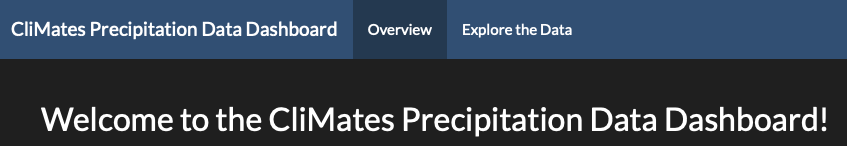
\includegraphics[width = .9\textwidth]{graphics/overview}
\end{center}


\begin{wrapfigure}{r}{.5\textwidth}

  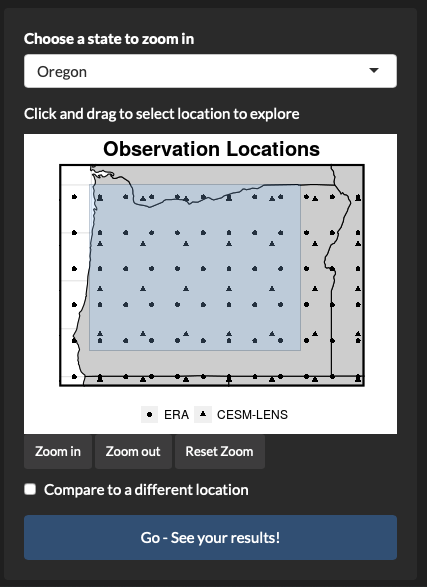
\includegraphics[width=.45\textwidth]{graphics/brushedpoints}
\end{wrapfigure}
The landing page of our app starts with a brief overview of the application, the application authors, and the materials used to make it (much of which is repeated in this report). The user then navigates to the “Explore the Data” tab to start.




There the user can decide what location they want to explore and the spatial scale at which to explore it. Since the authors (the CliMates) are based in Oregon, we’ll start there. The user selects the state of interest if they want to zoom in to a finer scale. Minor zoom adjustments can be made at this point.

 There are two sets of points: circles denote the grid points for the ERA-Interim dataset, while triangles denote the grid points for the CESM-LENS dataset. We can see here that the ERA-Interim data is at a much finer spatial scale. Different tabs rely on different datasets.


Now the user selects what area in the map to explore by clicking and dragging a rectangular selection of interest. Once the point selection is finalized, the user clicks “Go” and the selected plot is rendered for the subsetted data.



The user also has the option to compare to a different region by checking the “Compare to a different location” checkbox. Another map appears, and the user repeats the selection process described above. We enjoyed comparing eastern/western Oregon where the rain shadow effect plays a role in the amount of rainfall, as well as comparing Oregon to New Mexico, for example, where long term trends in cumulative precipitation are notably different.



\subsection*{Model Variability}

Since the goal of the CESM-LENS data is to be able to distinguish between climate change effects and internal climate variability, a topic of interest is the variation between different members of the ensemble model. Members of an ensemble model can be thought of as iterations of the same model, each with slightly different starting points. With the plots on this tab we explore that internal climate variability.

During the preprocessing stage each pair of latitude and longitude is treated individually. Data were reduced by calculating average precipitation for each day of the year in groupings of location, decade, and member. At this point, decade 9 (2000-2005) was eliminated due to not being a full decade. Next, the range (from all of the members) of these daily average precipitations was calculated for each location and  decade. The reasoning here is that these ranges can be used as a proxy for the variability between members. This marks the end of preprocessing and the next step of filtering is chosen by the user.

When the user selects a location, these ranges are averaged again to get one value over that entire spatial area of the bounding box. Distinction between decades is retained throughout. Then, the boxplot displays the distribution of these averaged range values over all of the days of the year for each decade. The smoothed plot retains the day of the year information and displays these values by day of the year for each decade. These values of average range are described as equating to variability between members over time, but the intent is to develop intuition about this variability rather than strictly trying to quantify it.




\subsection*{Decadal Cumulative Precipitation}

The tab labeled “Decadal Cumulative Precipitation” uses CESM-LENS to investigate trends in cumulative precipitation from 1921 to 2005, and to compare seasonality of precipitation between different locations. One of the challenges of doing an exploratory data analysis of precipitation is that it tends to be very noisy data. Precipitation can go from zero one day to an unusually high measurement the next day, back down to zero and then to a smaller non-zero measurement. This presents a challenge when attempting to get a rough idea of “when does it rain?” and “what are the long term trends in precipitation?” for a particular geographic area. Two ideas for working around this issue came to mind: calculating mean precipitation for a period of time, and looking instead at cumulative precipitation.

To reduce the variability of precipitation, this plot calculates the cumulative sum, then takes the mean across all the years in a given decade. Taking the average across a decade reduces the variability of the estimator, but sacrifices some of its specificity. The cumulative sum resets to zero on October 1st of each year, which was chosen since it’s the beginning of a water year \cite{usgs}. The first plot combines these variance reduction strategies to show the average cumulative precipitation for each decade.The user can zoom in by clicking and dragging to select an area of the plot, then double clicking to zoom in. This facilitates investigation into parts of the plot that would otherwise be difficult to read.

\begin{center}
  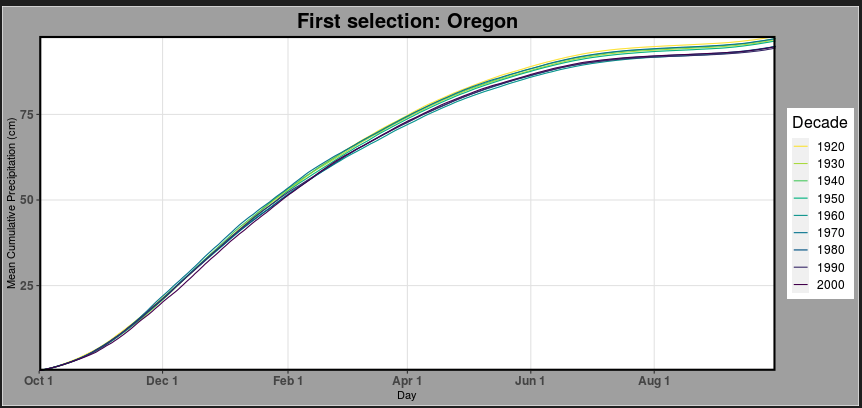
\includegraphics[width = .8\textwidth]{graphics/cumulative}
\end{center}



The second plot is the numeric derivative of the first plot. This shows what days of the year had the most rain. By comparing the two plots, it becomes clear how taking a cumulative sum reduces the noise. Calculating this as a numeric derivative rather than calculating the mean precipitation cuts down on the files that need to be stored and does not accrue enough computation time to significantly interfere with the user experience.

\begin{center}
  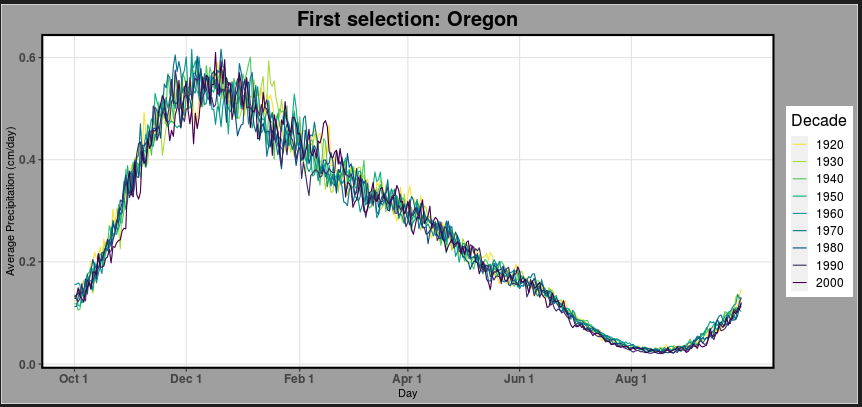
\includegraphics[width = .8\textwidth]{graphics/derivative}
\end{center}

\subsection*{Yearly}

The tab labeled “Yearly” uses the ERA-Interim data set to provide an opportunity for the user to explore yearly behavior of precipitation with plots of three measurements. On this tab, the user is given the choice of a range of years in addition to the sidebar choice of location of interest. The first plot depicts mean rainfall aggregated by year; all precipitation measured within the selected location boundary is added for the years chosen.

\begin{center}
  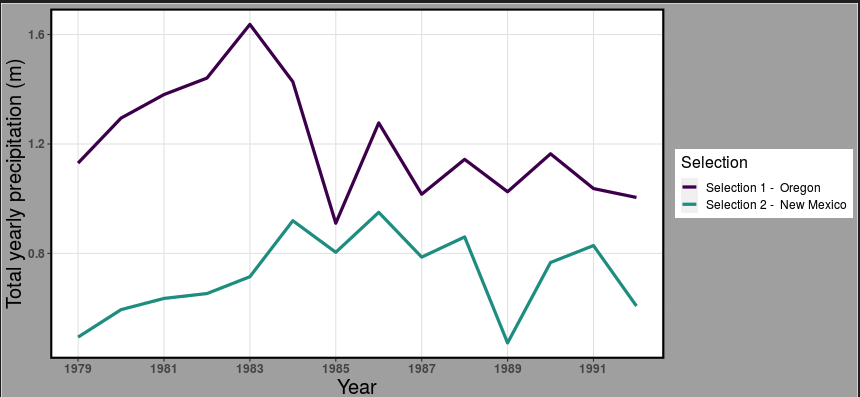
\includegraphics[width = .8\textwidth]{graphics/total}
\end{center}


The second plot portrays the cumulative precipitation for the location and range of years chosen; total yearly precipitation is cumulatively summed from the start to end year.

\begin{center}
  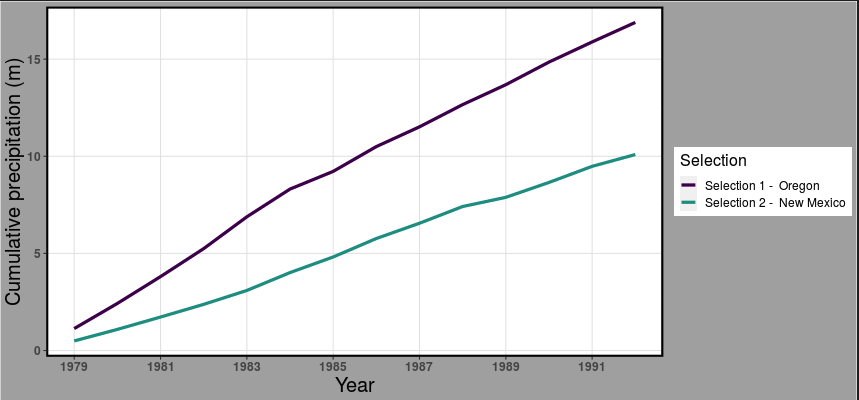
\includegraphics[width = .8\textwidth]{graphics/cumulative_year}
\end{center}

The third plot reveals the within-year variability of precipitation in the location of interest. This is calculated by finding the mean monthly precipitation for the location for all twelve months of the year and then calculating how these total values vary within the year. This allows the user to see how a year’s worth of precipitation values varies as a function of year.

\begin{center}
  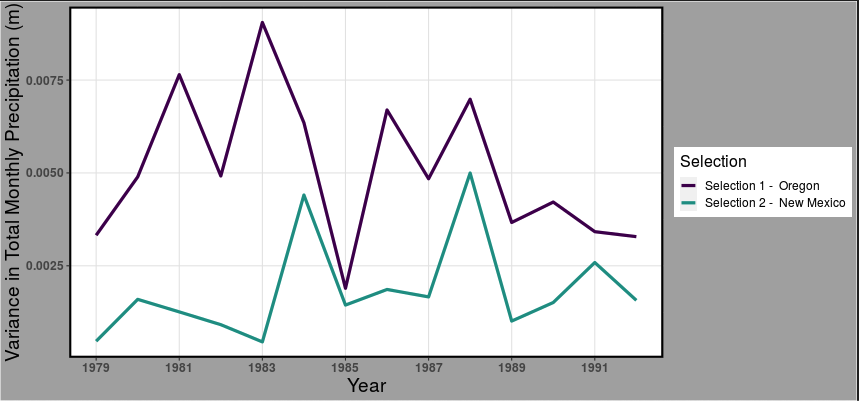
\includegraphics[width = .8\textwidth]{graphics/variance}
\end{center}

\subsection*{Seasonal Precipitation Deviation}

This tab allows users to explore trends at a seasonal level (winter/spring/summer/fall).  It explores the percent deviation in rainfall, calculated as the average seasonal precipitation for a given year and selected location, minus the average overall seasonal precipitation for the selected location, divided by the average overall seasonal precipitation at the selected location.  This tab is based on a pre aggregated dataset that is aggregated down to the seasonal level. Thus, for every grid point in the ERA-Interim dataset, there are four values per year.

The first plot shows a line chart breaking down these deviations by season. The overall United States average is included as a comparison (and the user can click the checkbox to remove this if wanted). If the user selected another region to compare there will be a third line on this chart.


The results of this tab are widely different depending on the selected location. Overall, for the United States average, we see that precipitation has been lower than average for the past 15 years or so. This trend is noisier and less pronounced when looking at the selected Oregon points. Other selected locations - South Dakota for instance, shows a much larger negative percent deviation in recent years, the most noticeably in summer months.

\begin{center}
  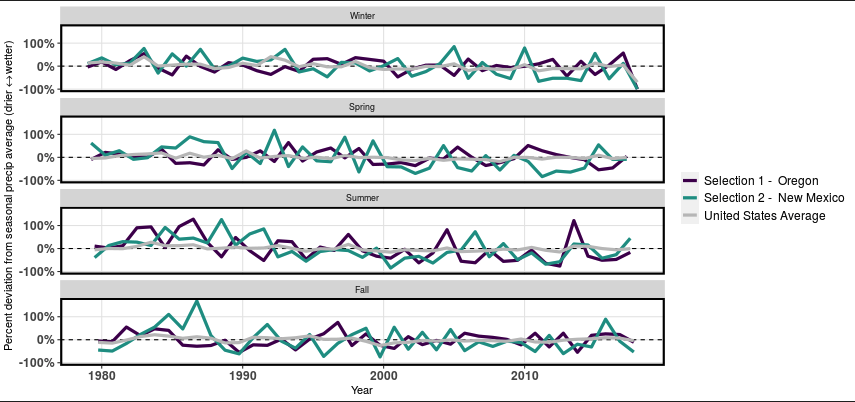
\includegraphics[width = .8\textwidth]{graphics/seasonal_deviation}
\end{center}

The second plot on this tab shows precipitation strips - inspired in part by the Warming/Climate stripes created by Ed Hawkins, Professor for Climate Science at the University of Reading \cite{hawkins}. Each strip represents the percent deviation from average precipitation values (described above). Brown stripes represent drier seasons, green stripes represent wetter seasons.This graphic shows that often drier periods last longer than a season, similarly for wetter periods. Some even last multiple years. Each row of this graphic is a different selected location, including the US average baseline. Often, periods of dry/wet happen at the same time for different locations/across the US.

\begin{center}
  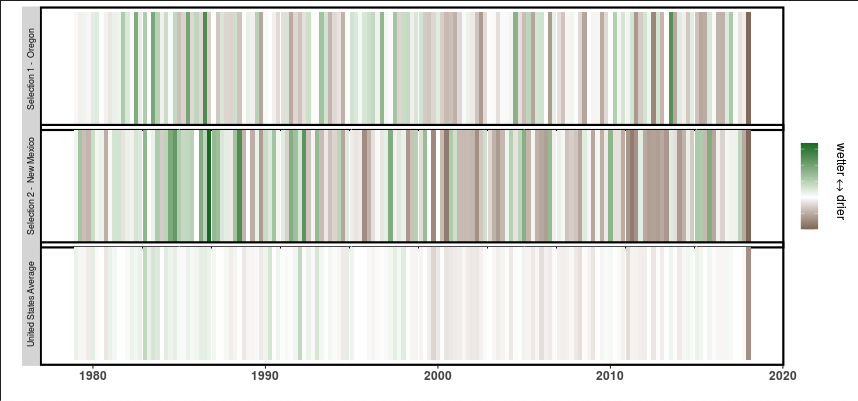
\includegraphics[width = .8\textwidth]{graphics/precipitation_strips}
\end{center}





\section*{Conclusion}

We were able to see interesting regional aspects of the data that were not able to be seen when aggregated across the entire spatial scale (all of the United States). Throughout our plots, we saw that times and locations with more rainfall were more variable in said rainfall. Even from selecting just a few locations using this EDA app, the authors came up with numerous questions from the observations in this app. We hope that this app is a helpful starting place for researchers interested in examining regional precipitation trends.


%\section*{Supporting information}

% Include only the SI item label in the paragraph heading. Use the \nameref{label} command to cite SI items in the text.


\section*{Acknowledgments}

We'd like to thank our faculty advisors for their support in this endeavor: Lisa Ganio PhD., James Molyneux, and Charlotte Wickham. Additionally, thank you to Jupiter Intelligence, the CESM Large Ensemble Community Project, and the European Centre for Medium-Range Weather Forecasts as well as the ASA ENVR Section for aggregating the data resources used in this effort. And, thank you to CJ Keist at OSU CoSINe IT Services for setting up and overseeing the RStudio server.
Thank you to the ASA Environmental Section for hosting this competition. The combination of R, Shiny, GitHub and large climate datasets used in this competition provided fun and challenging means for us to learn important tools in our field.




\nolinenumbers

% Either type in your references using
% \begin{thebibliography}{}
% \bibitem{}
% Text
% \end{thebibliography}
%
% or
%
% Compile your BiBTeX database using our plos2015.bst
% style file and paste the contents of your .bbl file
% here. See http://journals.plos.org/plosone/s/latex for
% step-by-step instructions.
%
\bibliography{mybibfile.bib}
% \begin{thebibliography}{10}

% \bibitem{bib1}
% Conant GC, Wolfe KH.
% \newblock {{T}urning a hobby into a job: how duplicated genes find new
%   functions}.
% \newblock Nat Rev Genet. 2008 Dec;9(12):938--950.
%
% \bibitem{bib2}
% Ohno S.
% \newblock Evolution by gene duplication.
% \newblock London: George Alien \& Unwin Ltd. Berlin, Heidelberg and New York:
%   Springer-Verlag.; 1970.
%
% \bibitem{bib3}
% Magwire MM, Bayer F, Webster CL, Cao C, Jiggins FM.
% \newblock {{S}uccessive increases in the resistance of {D}rosophila to viral
%   infection through a transposon insertion followed by a {D}uplication}.
% \newblock PLoS Genet. 2011 Oct;7(10):e1002337.
%
% \end{thebibliography}



\end{document}
